\documentclass[preview=true]{standalone}
\usepackage{tikz}
\usepackage{pgfplots}
\usepackage[siunitx, american]{circuitikz}
\usepackage[utf8]{inputenc}
\usepackage{newtxtext,newtxmath}
\usepackage[T1]{fontenc}
\pgfplotsset{compat=1.18}
\usepgfplotslibrary{units, fillbetween, smithchart, colormaps}
\usetikzlibrary{positioning, shapes, arrows, arrows.meta, graphs, shapes.geometric, math}
\tikzset{>=latex} % Better arrow tips

\begin{document}
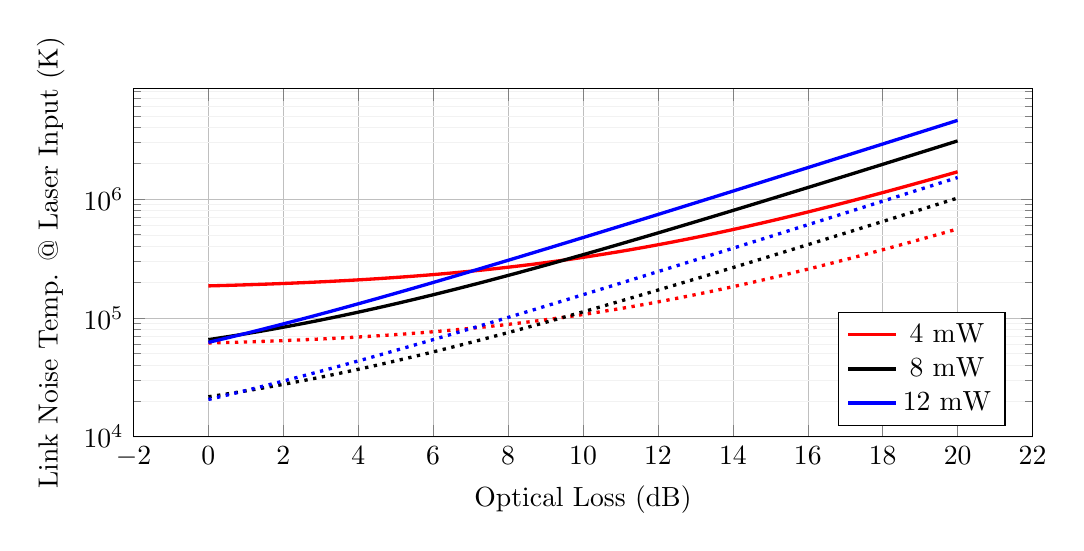
\begin{tikzpicture}[
    declare function={
        RIN(\P) = 10^((-131.2 - 5.5*(\P*1000) + 0.19*(\P*1000)^2)/10);
        Te(\P,\GOPT,\RS) = \P*\RS/(4*\KB*\SL^2*\GOPT*\ETAP) * (\P*\GOPT*\ETAP*RIN(\P) + 2*\Q) * (\RL/\RS + 1)^2;
    },
]

\newcommand\KB{1.380649e-23}
\newcommand\Q{1.60217663e-19}
\newcommand\ETAP{0.93}
\newcommand\SL{0.315}
\newcommand\RL{5}

\begin{axis}[width=13cm, height=6cm,
            grid={both}, 
            grid style={line width={.1pt}, 
            draw={gray!10}}, 
            major grid style={line width={.2pt}, draw={gray!50}},
            ymode=log,
            ymin = 10000,
            legend pos={south east},
            ylabel={Link Noise Temp. @ Laser Input (K)},
            xlabel={Optical Loss (dB)}]

    \addplot[color=red,
             domain=0:20, 
             samples=100,
             very thick]
    {
      Te(4e-3,10^(-x/10),50)
    };
    \addlegendentry{4 mW}
    \addplot[color=red,dotted,domain=0:20, samples=100,very thick,forget plot]
    {
      Te(4e-3,10^(-x/10),\RL)
    };

    \addplot[color=black,
             domain=0:20, 
             samples=100,
             very thick]
    {
      Te(8e-3,10^(-x/10),50)
    };
    \addlegendentry{8 mW}
    \addplot[color=black,dotted,domain=0:20, samples=100,very thick,forget plot]
    {
      Te(8e-3,10^(-x/10),\RL)
    };

    \addplot[color=blue,
             domain=0:20, 
             samples=100,
             very thick]
    {
     Te(12e-3,10^(-x/10),50)
    };
    \addlegendentry{12 mW}
    \addplot[color=blue,dotted,domain=0:20, samples=100,very thick,forget plot]
    {
      Te(12e-3,10^(-x/10),\RL)
    };
            
\end{axis}
\end{tikzpicture}
\end{document}